\section{Model Evaluation and Validation}

\subsection{Validation Framework}

To evaluate the performance of the models during training, the dataset was split into training and validation sets using a stratified split with a ratio of \textit{80:20}. The validation set was used to monitor performance during training and prevent overfitting:

\begin{minipage}{0.9\linewidth}\begin{lstlisting}[caption={Stratified split of the dataset into training and validation sets.},label={lst-train-vald-split}]
from sklearn.model_selection
    import train_test_split
from torch.utils.data import Subset

labels = [label for _, label
            in dataset.samples]
train_indices, val_indices = train_test_split(
    range(len(dataset)),
    test_size=0.2,
    stratify=labels,
    random_state=RANDOM_SEED,
)

train_dataset = Subset(dataset, train_indices)
val_dataset = Subset(dataset, val_indices)
\end{lstlisting}\end{minipage}

Since the dataset is imbalanced, a stratified split was used to ensure that the class distribution in the training and validation sets is similar. This prevents the model from overfitting the training set and ensures that it generalizes well to unseen data.

This split results in a training set of \textit{3800} and a validation set of \textit{950} samples (see~Fig.~\ref{fig:train-vald-split}).

\begin{figure}[htbp]
    \centerline{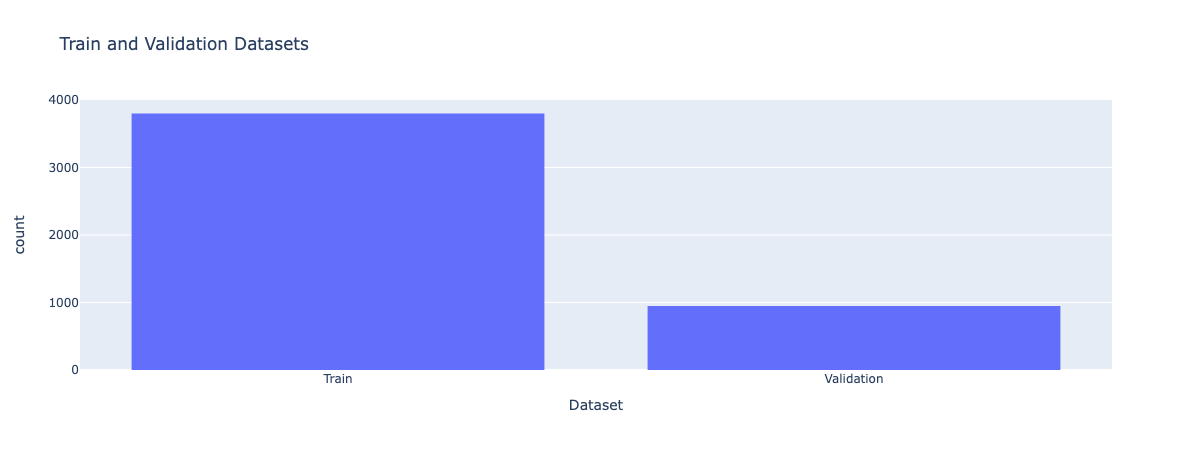
\includegraphics[width=0.9\linewidth]{../../resources/train_vald_split.png}}
    \caption{Training and validation set sizes}
    \label{fig:train-vald-split}
\end{figure}

Since there are no labels for the test set, the validation set serves as a proxy to evaluate the performance of the model on unseen data (not used during training). Validation loss and accuracy were monitored during training to assess the convergence and generalization capabilities of the models:

\begin{figure}[htbp]
    \centerline{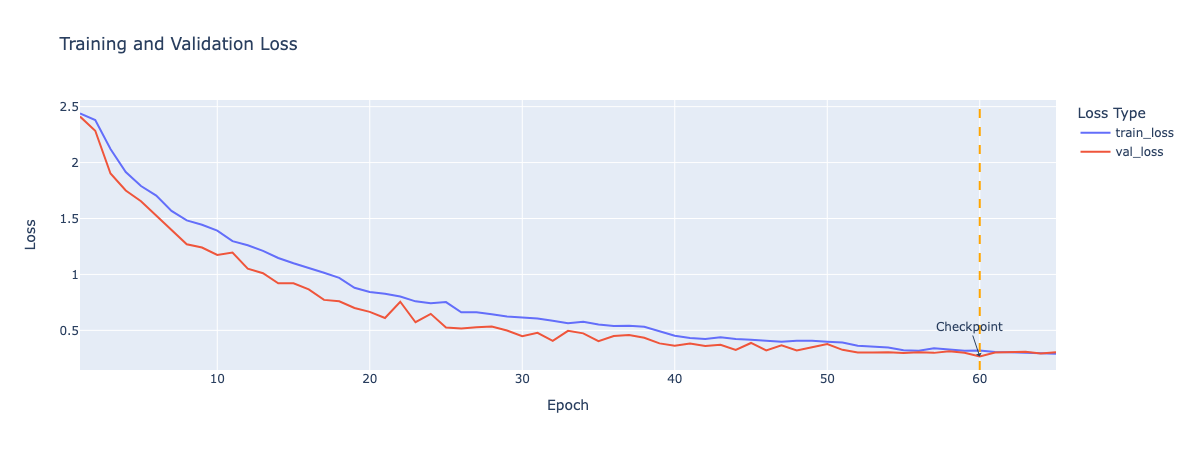
\includegraphics[width=0.9\linewidth]{../../resources/custom_cnn/loss.png}}
    \caption{Training and validation loss~(custom CNN)}
    \label{fig:loss-custom-cnn}
\end{figure}

\begin{figure}[htbp]
    \centerline{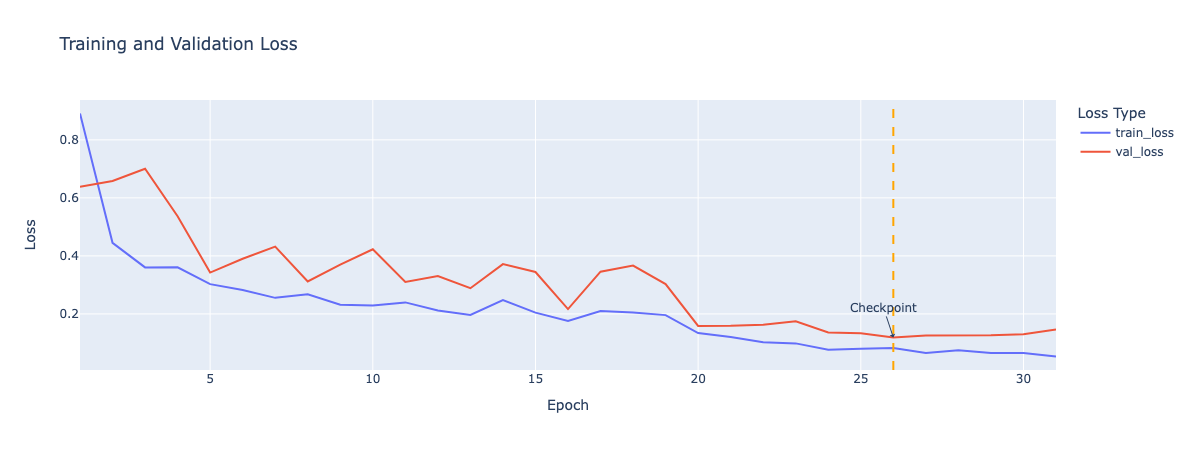
\includegraphics[width=0.9\linewidth]{../../resources/resnet/loss.png}}
    \caption{Training and validation loss~(pre-trained CNN)}
    \label{fig:loss-pretrained-cnn}
\end{figure}

\begin{figure}[htbp]
    \centerline{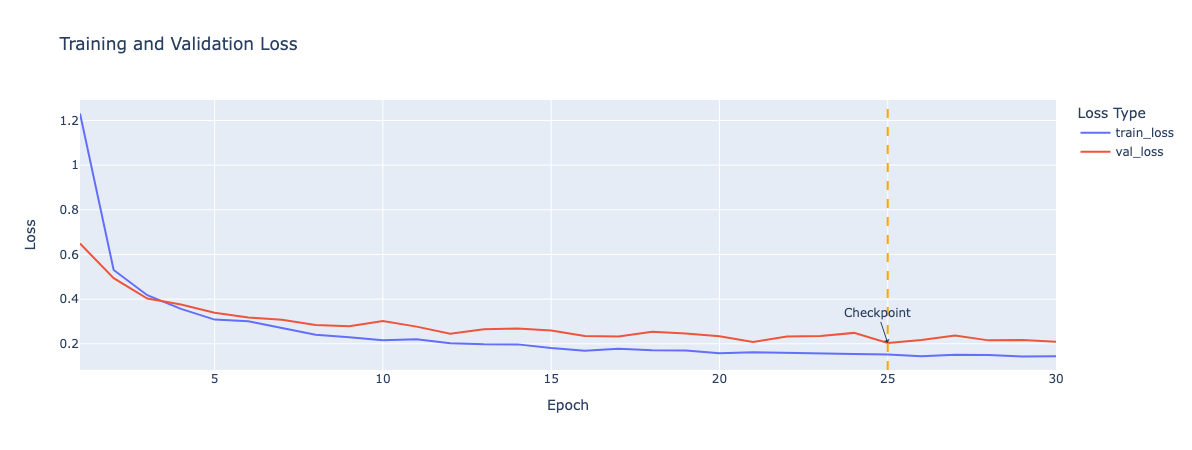
\includegraphics[width=0.9\linewidth]{../../resources/vit/loss.png}}
    \caption{Training and validation loss~(pre-trained ViT)}
    \label{fig:loss-pretrained-vit}
\end{figure}

Fig.~\ref{fig:loss-custom-cnn}, Fig.~\ref{fig:loss-pretrained-cnn} and Fig.~\ref{fig:loss-pretrained-vit} show the training and validation loss curves for the custom CNN, pre-trained CNN and pre-trained ViT models, respectively. Each curve illustrates the learning dynamics of the model over successive epochs.

The custom CNN demonstrates a gradual reduction in both training and validation loss, converging steadily around epoch \textit{60}. This indicates effective learning without overfitting, as the training and validation loss curves remain closely aligned. One could argue that the model could benefit from increased complexity and further training to improve performance.

The pre-trained CNN shows faster convergence, with training and validation loss stabilizing around epoch \textit{26}. This faster convergence reflects the advantages of fine-tuning, as the model uses pre-trained weights for feature extraction. Similarly, the pre-trained ViT, which also converges rapidly within \textit{25} epochs, demonstrates the effectiveness of using pre-trained models and transfer learning for this classification task. However the gap between training and validation loss suggests that the model could benefit from additional regularization to improve generalization. In particular, the pre-trained CNN begins to clearly overfit the data after epoch \textit{30}.

The inclusion of a checkpoint in each figure highlights the point at which the model achieved the lowest validation loss, indicating optimal performance and serving as a reference for saving the best model state. The loaded checkpoints are at epoch \textit{60}, \textit{26} and \textit{25} for the custom CNN, pre-trained CNN and pre-trained ViT, respectively.

\subsection{Performance Metrics}

In addition to losses, validation accuracy is tracked during training to monitor performance of the models. Accuracy is calculated as the ratio of correctly predicted samples to the total number of samples in the validation set:

\begin{equation}
    \text{Accuracy} = \frac{\text{Number of Correct Predictions}}{\text{Total Number of Samples}}\label{eq:accuracy}
\end{equation}

The accuracy~(\ref{eq:accuracy}) provides a simple and intuitive measure of performance on the validation set:

\begin{figure}[htbp]
    \centerline{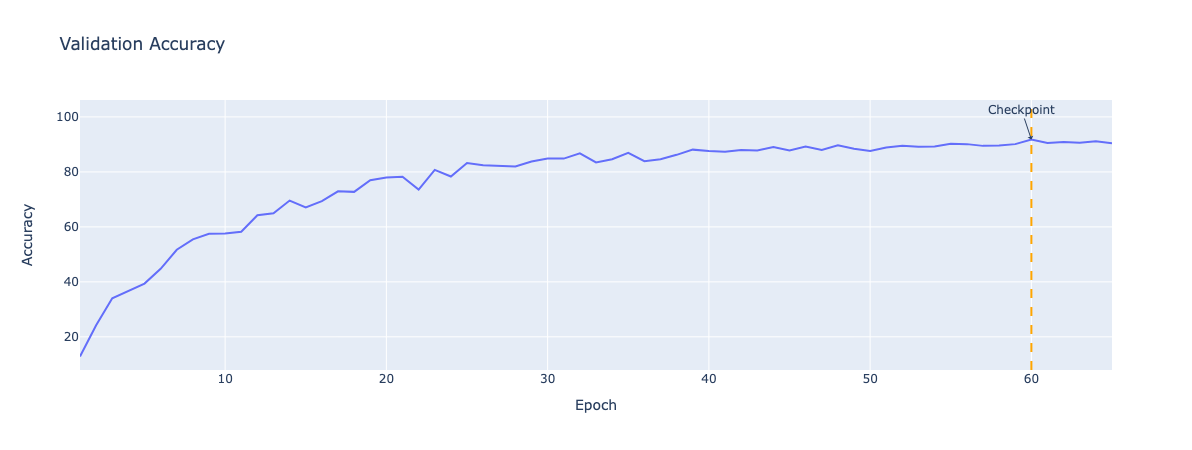
\includegraphics[width=0.9\linewidth]{../../resources/custom_cnn/accuracy.png}}
    \caption{Validation accuracy~(custom CNN)}
    \label{fig:accuracy-custom-cnn}
\end{figure}

\begin{figure}[htbp]
    \centerline{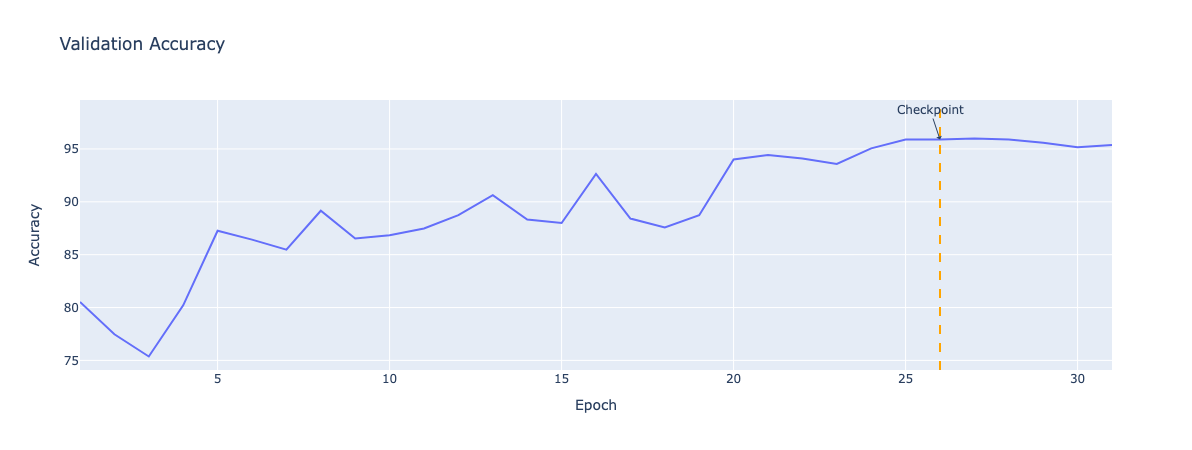
\includegraphics[width=0.9\linewidth]{../../resources/resnet/accuracy.png}}
    \caption{Validation accuracy~(pre-trained CNN)}
    \label{fig:accuracy-pretrained-cnn}
\end{figure}

\begin{figure}[htbp]
    \centerline{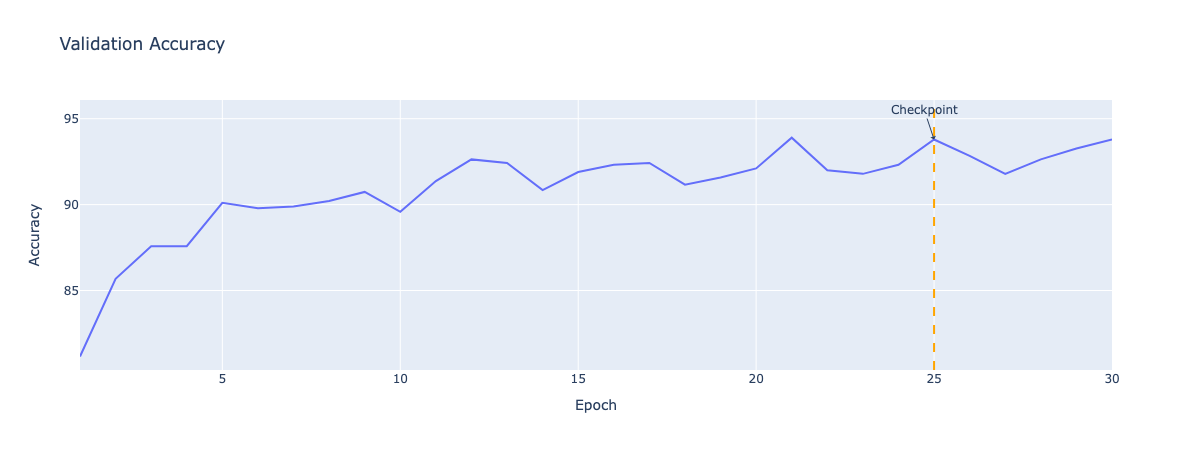
\includegraphics[width=0.9\linewidth]{../../resources/vit/accuracy.png}}
    \caption{Validation accuracy~(pre-trained ViT)}
    \label{fig:accuracy-pretrained-vit}
\end{figure}

Similar to the loss curves, Fig.~\ref{fig:accuracy-custom-cnn}, Fig.~\ref{fig:accuracy-pretrained-cnn} and Fig.~\ref{fig:accuracy-pretrained-vit} show the validation accuracy of the custom CNN, pre-trained CNN and pre-trained ViT models, respectively. The accuracy curves provide insight into the ability of the model to correctly classify the validation samples over successive epochs. The figures highlight the information from the loss curves, showing that the pre-trained models converge faster and achieve higher accuracy compared to the custom CNN. But again, the custom CNN shows a steady and smooth increase in accuracy over time, indicating that the model continues to learn and improve its performance. The selected checkpoints are the same as for the loss curves, indicating the load state of the model with the lowest validation loss, which also corresponds to high accuracy.